\documentclass[a4paper,14pt]{extreport}
\usepackage[left=1.5cm,right=1.5cm,
    top=1.5cm,bottom=2cm,bindingoffset=0cm]{geometry}
\usepackage{diagbox}
\usepackage{nicematrix,tikz}
\usetikzlibrary{fit}

\usepackage{scrextend}

	
	\usepackage{amsmath,amssymb}
	\usepackage{array,tabularx}
	\usepackage{graphicx}
	\graphicspath{{C:/Users/anmnm/Desktop/TeX/images/}}
	\usepackage{moreverb}
	\usepackage{xcolor}
	\usepackage{color}
	\usepackage{hyperref}
	\hypersetup{%
		colorlinks=true,
		linkbordercolor= red,
		urlbordercolor=green,
    }%for hyperrefs
%------------------ 
\usepackage[many]{tcolorbox}
	\newtcbox{\mylib}{enhanced,nobeforeafter,tcbox raise base,boxrule=0.4pt,top=0mm,bottom=0mm,
	  right=0mm,left=4mm,arc=1pt,boxsep=2pt,before upper={\vphantom{dlg}},
	  colframe=green!50!black,coltext=green!25!black,colback=green!10!white,
	  overlay={\begin{tcbclipinterior}\fill[green!75!blue!50!white] (frame.south west)
	    rectangle node[text=white,font=\sffamily\bfseries\tiny,rotate=90] {TYP} ([xshift=4mm]frame.north west);\end{tcbclipinterior}}}

%------------------  
\newcolumntype{Y}{>{\centering\arraybackslash}X}
%------------------  
\usepackage{lstautogobble}  % Fix relative indenting
\usepackage{color}          % Code coloring
\usepackage{zi4}            % Nice font
	\definecolor{bluekeywords}{rgb}{0.13, 0.13, 1}
	\definecolor{greencomments}{rgb}{0, 0.5, 0}
	\definecolor{redstrings}{rgb}{0.9, 0, 0}
	\definecolor{graynumbers}{rgb}{0.5, 0.5, 0.5}

	\usepackage{listings}
	\lstset{
  basicstyle=\ttfamily,
  columns=fullflexible,
  frame=single,
  breaklines=true,
  postbreak=\mbox{\textcolor{red}{$\hookrightarrow$}\space},
  }
%------------------
\usepackage[object=vectorian]{pgfornament} %%  http://altermundus.com/pages/tkz/ornament/index.html
		\usepackage{tikz}
		\newcommand{\sectionlinetwo}[2]{%
		\nointerlineskip \vspace{.5\baselineskip}\hspace{\fill}
		{\color{#1}
		\resizebox{0.5\linewidth}{2ex}
		{{{\begin{tikzpicture}
		\node  (C) at (0,0) {};\node (D) at (9,0) {};
		\path (C) to [ornament=#2] (D);
		\end{tikzpicture}}}}}%
		\hspace{\fill}
		\par\nointerlineskip \vspace{.5\baselineskip}}

  %\newcommand{\img}[4]{\center{\includegraphics[width=#1\linewidth]{#2}}\captionof{figure}{#3}\label{#4}}
\newcommand{\img}[4]{\includegraphics[width=#1\linewidth]{#2}\caption{#3}\label{#4}}


%-----------------------------
\usepackage{tcolorbox}
\tcbuselibrary{skins,breakable}
\usetikzlibrary{shadings,shadows}%preambule
%-----------------------------
\newtcbox{\mybox}[1][red]{on line,
arc=0pt,outer arc=0pt,colback=#1!10!white,colframe=#1!50!black,
boxsep=0pt,left=1pt,right=1pt,top=2pt,bottom=2pt,
boxrule=0pt,bottomrule=1pt,toprule=1pt}

\newtcbox{\xmybox}[1][red]{on line,
arc=7pt,colback=#1!10!white,colframe=#1!50!black,
before upper={\rule[-3pt]{0pt}{10pt}},boxrule=1pt,
boxsep=0pt,left=6pt,right=6pt,top=2pt,bottom=2pt}
%-----------------------------
\usepackage{tikz}
\usetikzlibrary{shapes.callouts}
%-----------------------------
\definecolor{amber}{rgb}{1.0, 0.75, 0.0}
\definecolor{babyblue}{rgb}{0.54, 0.81, 0.94}
%-----------------------------

	\usepackage[framemethod=TikZ]{mdframed}
	\usetikzlibrary{calc}
	\makeatletter
	\newlength{\mylength}
	\xdef\CircleFactor{1.1}
	\setlength\mylength{\dimexpr\f@size pt}
	\newsavebox{\myboxx}
	\newcommand*\circled[2][draw=blue]{\savebox\myboxx{\vbox{\vphantom{WL1/}#1}}\setlength\mylength{\dimexpr\CircleFactor\dimexpr\ht\myboxx+\dp\myboxx\relax\relax}\tikzset{mystyle/.style={circle,#1,minimum height={\mylength}}}
	\tikz[baseline=(char.base)]
	\node[mystyle] (char) {#2};}
	\makeatother
%-----------------------------
\usepackage{verbatim}

\usetikzlibrary{arrows,shapes,backgrounds}
%-----------------------------
\usepackage{multicol}
%-----------------------------
%\usepackage[most]{tcolorbox}
	\definecolor{orang}{RGB}{255,155,0}
	\newtcolorbox[auto counter,number within=section]{caja}[1][]{
	enhanced jigsaw,colback=white,colframe=orang,coltitle=orang,
	fonttitle=\bfseries\sffamily,
	sharp corners,
	detach title,
	leftrule=10mm,
	% What you need %%%%%%%%%%%%
	underlay unbroken and first={\node[below,text=black,anchor=east]
	at ([xshift=-5.5pt]interior.base west) {\Huge  \textbf{!}};},
	%%%%%%%%%%%%%%%%%%%%%%%%
	breakable,pad at break=1mm,
	#1,
	code={\ifdefempty{\tcbtitletext}{}{\tcbset{before upper={\tcbtitle\par\medskip}}}},}
%-----------------------------
%-----------------------------
%-----------------------------
%-----------------------------
%-----------------------------
%-----------------------------
%-----------------------------
%-----------------------------
%-----------------------------
%-----------------------------
%-----------------------------

\begin{document}
\renewcommand{\bibname}{Список використаної літератури}% -- переименуем название списка литературы
\begin{titlepage}
  \begin{center}
  {\large МІНІСТЕРСТВО ОСВІТИ І НАУКИ УКРАЇНИ}\\[0.2cm]
{\large НАЦІОНАЛЬНИЙ ТЕХНІЧНИЙ УНІВЕРСИТЕТ УКРАЇНИ}\\[0.2cm]
 {\large <<КИЇВСЬКИЙ ПОЛІТЕХНІЧНИЙ ІНСТИТУТ>>}

\vspace{1cm}
  {\large Факультет Електроніки}\\[0.3cm]

  {\large Кафедра мікроелектроніки}
  
\vspace{2cm}
  {\Large КУРСОВИЙ ПРОЕКТ (РОБОТА)} \\
  {\large з дисципліни: <<Схемотехніка-3>>}\\[1cm]
    
\bigskip
  \end{center}
  


\begin{center}
\begin{tabular}{ll}
Керівник:&\hspace{1cm}Виконав:\\[0.2cm]
Ніколов Микола Олександрович&\hspace{1cm}Студент 4-го курсу, групи ДП-82\\[0.5cm]
“Допущений до захисту”&\hspace{1cm} Мнацаканов Антон Станіславович\\[0.5cm]
$\underset{\text{(особистий підпис керівника)}}{\underline{\hspace{0.433\textwidth}}}$&\hspace{1cm}Залікова книжка № $\underset{}{\underline{\hspace{0.15\textwidth}}}$\\[0.5cm]
Захищений з оцінкою $\underset{\text{(особистий підпис)}}{\underline{\hspace{0.15\textwidth}}}$&\text{}\\[0.5cm]
$\underset{\text{(особистий підпис)(ПІБ)}}{\underline{\hspace{0.433\textwidth}}}$ &\text{}\\[0.5cm]
$\underset{\text{(особистий підпис)(ПІБ)}}{\underline{\hspace{0.433\textwidth}}}$ &\text{}\\[0.5cm]
$\underset{\text{(особистий підпис)(ПІБ)}}{\underline{\hspace{0.433\textwidth}}}$&\text{}
\end{tabular}
\end{center}

\vfill

\begin{center}
Київ – 2021
\end{center}
\end{titlepage}
%%%%%%%%%%%%%%%%%%%%%%%%%%%%%%%%%%%%%%%%%%%%%%%%%%%%%%%%%%%%%%%%%%%%%%%%%%%%%%%%%%%%%%%%%%
\tableofcontents
%%%%%%%%%%%%%%%%%%%%%%%%%%%%%%%%%%%%%%%%%%%%%%%%%%%%%%%%%%%%%%%%%%%%%%%%%%%%%%%%%%%%%%%%%%

\chapter{ЗАВДАННЯ }
  %\section{Подраздел}
  \begin{enumerate}
  \item  Вибрати тип тригерів відповідно до варіанта.
\item Побудувати таблицю станів згідно з варіантом.
\item Синтезувати лічильник згідно з таблицею станів. Забезпечити встановлення початкового стану за зовнішнім сигналом СКИДАННЯ (активний рівень «1»). Полярність сигналу синхронізації вибрати згідно з таблицею 3.
\item Розробити важливу електричну схему лічильника.
\item Провести аналіз роботи розробленої схеми, відобразити послідовності логічних рівнів кожного такту на виходах лічильника і виходах комбінаційних логічних елементів схеми.
\item Побудувати часові діаграми, що відображають роботу лічильника з урахуванням затримок (проілюструвати всю лічильну послідовність).
  \end{enumerate}
Моя послідовність: 7 8 9 10 11 12 13 1 15 0 14 2 3 4 5 6.\\ 

Згенерована послідовність містить 16 цифр, тому коефіцієнт $\text{К}_{\text{сч}} = 16$. Формула для розрахунку тригерів n, необхідна для синтезу лічильника є ніщо інше як двійковий логарифм $\text{К}_{\text{сч}}$, округлена в більшу сторону:

\begin{equation}
n = \log_2\text{К}_{\text{сч}}.
\end{equation}

З цієї рівності видно, що для синтезу лічильника нам знадобиться 4 тригери.
Для підвищення швидкодії цифрового пристрою буде використовуватись синхронний паралельний лічильник, тобто він матиме одну спільну для всіх шину синхронізації, тому тригери будуть перемикатись синхронно по передньому фронту генератора лічильних імпульсів, як вказано в умові.\\



 Для правильної роботи синхронного паралельного лічильника на всі синхровходи потрібно одночасно подавати синхроімпульс. На JK входи першого розряду потрібно подавати логічну одиницю, для цього ми буде використовувати джерело напруги (VCC). На JK входи другого розряду потрібно подати прямий вихід тригера першого розряду. На JK входи наступних розрядів потрібно подавати кон'юнкцію прямих виходів тригерів попередніх розрядів.

\begin{figure}[h!]
\img{0.7}{qwe.pdf}{Прототип лічильника}{s2}
\end{figure}

 %%%%%%%%%%%%%%%%%%%%%%%%%%%%%%%%%%%%%%%%%%%%%%%%%%%%%%%%%%%%%%%%%%%%%%%%%%%%%%%%%%%%%%%%%%
\chapter{  ТАБЛИЦЯ СТАНIВ   }
\begin{table}[h!]

\begin{center}


\begin{tabular}{c|ccccc|ccccc|c}
K && $Q_{3}$ & $Q_{2}$ & $Q_{1}$ & $Q_{0}$ & $  y_{3}$ & $y_{2}$ & $y_{1}  $ & $y_{0}$&& K\\
 0 && 0 & 0 & 0 & 0 & 0 & 1 & 1 & 1   &&7 \\
1 && 0 & 0 & 0 & 1 & 1 & 0 & 0 & 0 &&  8  \\
2 && 0 & 0 & 1 & 0 & 1 & 0 & 0 & 1 &&  9  \\
3 && 0 & 0 & 1 & 1 & 1 & 0 & 1 & 0 &&  10 \\
4 && 0 & 1 & 0 & 0 & 1 & 0 & 1 & 1 &&  11 \\
5 && 0 & 1 & 0 & 1 & 1 & 1 & 0 & 0 &&  12 \\
6 && 0 & 1 & 1 & 0 & 1 & 1 & 0 & 1 &&  13 \\
7 && 0 & 1 & 1 & 1 & 0 & 0 & 0 & 1 &&  1  \\
8 && 1 & 0 & 0 & 0 & 1 & 1 & 1 & 1 &&  15 \\
9 && 1 & 0 & 0 & 1 & 0 & 0 & 0 & 0 &&  0  \\
10&& 1 & 0 & 1 & 0 & 1 & 1 & 1 & 0 &&  14 \\
11&& 1 & 0 & 1 & 1 & 0 & 0 & 1 & 0 &&  2  \\
12&& 1 & 1 & 0 & 0 & 0 & 0 & 1 & 1 &&  3  \\
13&& 1 & 1 & 0 & 1 & 0 & 1 & 0 & 0 &&  4  \\
14&& 1 & 1 & 1 & 0 & 0 & 1 & 0 & 1 &&  5  \\
15&& 1 & 1 & 1 & 1 & 0 & 1 & 1 & 0 &&  6  \\
\end{tabular}

\caption{Таблиця істинності }
\end{center}
\end{table}
\vspace{1cm}
Будуємо по цій таблиці карти Карно.\\ 

%%%%%%%%%%%%%%%%%%%%%%%%%%%%%%      1        %%%%%%%%%%%%%%%%%%%%%%%%%%%%%%%%%
  \begin{minipage}[h!]{0.4\linewidth} 
    $y_0$ \fcolorbox{red}{white}{I}, \fcolorbox{green}{white}{II}, \fcolorbox{blue}{white}{III}, \fcolorbox{black}{white}{IV} \\[0.2 cm]
   \begin{NiceTabular}{|p{1.2cm}|c|c|c|c|}
  \hline
   \diagbox{\footnotesize{$Q_3 Q_2$}}{\footnotesize{$Q_1 Q_0$}} & 00 & 01 & 11 & 10  \\\hline
               00                                               &  1   & 0  &  0  &1\\\hline
               01                                               &   1  & 0  &  1   &1\\\hline
               11                                               &   1  & 0  &  0  &1\\\hline
               10                                               &  1   & 0  &  0  & 0 \\ \hline

  \CodeAfter 
    \tikz \node [draw=red,rounded corners,fit=(5-4)(5-5)] {} ; %1
    \tikz \node [draw=green,rounded corners,fit=(2-3)(2-4)] {} ; %2
    \tikz \node [draw=green,rounded corners,fit=(5-3)(5-4)] {} ; %2
    \tikz \node [draw=blue,rounded corners,fit=(4-3)(5-4)] {} ; %3
    \tikz \node [draw=black,rounded corners,fit=(2-3)(5-3)] {} ; %4

  \end{NiceTabular}
  \end{minipage}
  \hfill
  \begin{minipage}[m]{0.4\linewidth}
  \begin{align*}
  y_0 &= (\bar Q_3 +Q_2+\bar Q_1)\times  \\
  &\times (Q_2+\bar Q_0)\times (\bar Q_3 +\bar Q_0)\times \\ 
   & \times(Q_1 + \bar Q_0)
  \end{align*}
  \end{minipage}

\vspace{1cm}

%%%%%%%%%%%%%%%%%%%%%%%%%%%%%%      2        %%%%%%%%%%%%%%%%%%%%%%%%%%%%%%%%%
  \begin{minipage}[h!]{0.5\linewidth} 
    $y_1$ \fcolorbox{red}{white}{I}, \fcolorbox{green}{white}{II}, \fcolorbox{blue}{white}{III}, \fcolorbox{black}{white}{IV} \\[0.2 cm]
   \begin{NiceTabular}{|p{1.2cm}|c|c|c|c|}
  \hline
   \diagbox{\footnotesize{$Q_3 Q_2$}}{\footnotesize{$Q_1 Q_0$}} & 00 & 01 & 11  & 10  \\\hline
               00                                               &  1   & 0  &  1  & 0\\\hline
               01                                               &  1   & 0  &  0 & 0\\\hline
               11                                               & 1   & 0  &  1  & 0\\\hline
               10                                               &  1   & 0  &  1  & 1 \\ \hline

  \CodeAfter 
    \tikz \node [draw=red,rounded corners,fit=(3-5)(4-5)] {} ; %1
    \tikz \node [draw=green,rounded corners,fit=(2-5)(3-5)] {} ; %2
    \tikz \node [draw=blue,rounded corners,fit=(3-4)(3-5)] {} ; %3
    \tikz \node [draw=black,rounded corners,fit=(2-3)(5-3)] {} ; %4

  \end{NiceTabular}
  \end{minipage}
  \hfill
  \begin{minipage}[m]{0.4\linewidth}
  \begin{align*}
  y_1 &= (\bar Q_1 +Q_0+\bar Q_2)\times  \\
  &\times (\bar Q_1+Q_0+Q_3)\times (  Q_3 +\bar Q_2 + Q_1)\times  \\ 
  &\times(Q_1 + \bar Q_0)
  \end{align*}
  \end{minipage}

\vspace{1cm}

%%%%%%%%%%%%%%%%%%%%%%%%%%%%%%      3        %%%%%%%%%%%%%%%%%%%%%%%%%%%%%%%%%
  \begin{minipage}[h!]{0.4\linewidth} 
    $y_2$ \fcolorbox{red}{white}{I}, \fcolorbox{green}{white}{II}, \fcolorbox{blue}{white}{III}, \fcolorbox{black}{white}{IV} \\[0.2 cm]
   \begin{NiceTabular}{|p{1.2cm}|c|c|c|c|}
  \hline
   \diagbox{\footnotesize{$Q_3 Q_2$}}{\footnotesize{$Q_1 Q_0$}} & 00  & 01 & 11 & 10  \\\hline
               00                                               &  1   & 0  & 0   & 0\\\hline
               01                                               &  0  & 1  &  0 & 1 \\\hline
               11                                               &  0  &  1  & 1   & 1 \\\hline
               10                                               &  1   & 0  &  0  & 1 \\ \hline

  \CodeAfter 
    \tikz \node [draw=red,rounded corners,fit=(2-4)(2-5)] {} ; %1
    \tikz \node [draw=green,rounded corners,fit=(2-4)(3-4)] {} ; %2
    \tikz \node [draw=blue,rounded corners,fit=(3-2)(4-2)] {} ; %3
    \tikz \node [draw=black,rounded corners,fit=(2-3)(2-4)] {} ; %4
    \tikz \node [draw=black,rounded corners,fit=(5-3)(5-4)] {} ; %4

  \end{NiceTabular}
  \end{minipage}
  \hfill
  \begin{minipage}[m]{0.4\linewidth}
  \begin{align*}
  y_2 &= (  Q_3 + Q_2 + \bar Q_1)\times  \\
  &\times (\bar Q_1+\bar Q_0+Q_3)\times (  Q_1 + Q_0 + \bar Q_2)\times \\ 
  & \times(\bar Q_0 +Q_2 )
  \end{align*}
  \end{minipage}

\vspace{1cm}

%%%%%%%%%%%%%%%%%%%%%%%%%%%%%%      4        %%%%%%%%%%%%%%%%%%%%%%%%%%%%%%%%%
  \begin{minipage}[h!]{0.4\linewidth} 
    $y_3$ \fcolorbox{red}{white}{I}, \fcolorbox{green}{white}{II}, \fcolorbox{blue}{white}{III}, \fcolorbox{black}{white}{IV} \\[0.2 cm]
   \begin{NiceTabular}{|p{1.2cm}|c|c|c|c|}
  \hline
   \diagbox{\footnotesize{$Q_3 Q_2$}}{\footnotesize{$Q_1 Q_0$}} & 00  & 01  & 11  & 10  \\\hline
               00                                               &  0   & 1   &  1   &1 \\\hline
               01                                               &  1    &  1  &  0  & 1 \\\hline
               11                                               &  0   & 0  &  0  & 0 \\\hline
               10                                               &  1    & 0  &  0  &1  \\ \hline

  \CodeAfter 
    \tikz \node [draw=red,rounded corners,fit=(2-2)] {} ; %1
    \tikz \node [draw=green,rounded corners,fit=(4-2)(4-5)] {} ; %2
    \tikz \node [draw=blue,rounded corners,fit=(3-4)(4-4)] {} ; %3
    \tikz \node [draw=black,rounded corners,fit=(4-3)(5-4)] {} ; %4


  \end{NiceTabular}
  \end{minipage}
  \hfill
  \begin{minipage}[m]{0.6\linewidth}
  \begin{align*}
  y_3 &= (  Q_3 + Q_2 +   Q_1 + Q_0)\times  \\
  &\times (\bar Q_3+\bar Q_2)\times (  \bar Q_2 + \bar Q_1 + \bar Q_0) \times \\
  & \times(\bar Q_3 + \bar Q_0 )
  \end{align*}
  \end{minipage}





\chapter{  РЕЗУЛЬТАТИ   }
%%%%%%%%%%%%%%%%%%%%%%%%%%%%%%%%%%%%%%%%%%%%%%%%%%%%%%%%%%%%%%%%%%%%%%%%%%%%%%%%%%%%%%%%%%
 
Проведемо короткий аналіз отриманий залежностей. Основною елементною базою в нас виступатимуть диз'юнктори. Лише для розряду у3 нам знадобиться один чотрирьохвходовий диз'юнктор, а так вцілому у нас для кожного тригера число пінів для диз'юнктора не перевищує трьох. Натомість для кожного розряду нам знадобиться по одному чотирьохвходовому кон'юнктору. Звісно це трохи громіздко, але варто зазначити, що деякі множники розрядів в нас повторюються, тому ми можемо не городити зайвий раз логічні вентилі, що безумовно нівелює недолік з чотриривходовими кон'юнкторами.

\begin{figure}[h!]
\img{0.9}{sxema.png}{Електрична схема лічильника}{s1}
\end{figure}


\chapter{  ЧАСОВI ДIАГРАМИ  }
Для перевірки правильності функціонування лічильника побудуємо часові діаграми.


\begin{figure}[h!]
\img{0.9}{12.jpg}{Загальна часова діаграма роботи лічильника}{}
\end{figure}

\begin{figure}[h!]
\img{0.9}{123.jpg}{Часова діаграма роботи лічильника з новою послідовністю}{}
\end{figure}







\begin{thebibliography}{2}
\bibitem  hhttps://drive.google.com/file/d/1ZPkrN6ysmc060UY2x5C1yw-elpEHIgkO/view?usp=sharing\\
\bibitem  BB.И. Зубчук, В.П. Сигорский, А.Н. Шкуро. Справочник по цифровой схемотехнике \\
\bibitem   hhttps://drive.google.com/drive/folders/1GqdPdiKwwk-MPEQBbYbB9bHX91NX76xP
\end{thebibliography}


\chapter{   ВИСНОВОК }
В цій роботі було сформовано та змодельовано лічильник на JK-тригерах, який на мою думку є найбільш простим порівняно з D- або RS-тригерами. В даному випадку потрібро було розрахувати лише 16 цифр (0-15), для чого знадобилося лише 4 тригери. Судячи  з часових діаграм можна сказати що синтезований лічильник працює коректно -- це також підтверджується комп'ютерним моделюванням яке було проведено в програмі Multisim, в якій було  продемонстровано як загоряються світлодіоди з певною послідовністю. \\ 

Також що стосується часових діаграм, то я їх трішки ідеалізував, оскільки в реальності кожний вентиль трішки, але все ж таки вносить свою затримку для сигналу, але оскільки все було зроблено та просимульовано в ідеальних умовах, тобто впрограмі то і результати я вирішив зробити більш нашлядними, але в реальних умовах ці діаграми будуть більш схожі на трапеції а не на прямокутники. 


\chapter{   ДОДАТОК А  }
 


\begin{figure}[h!]
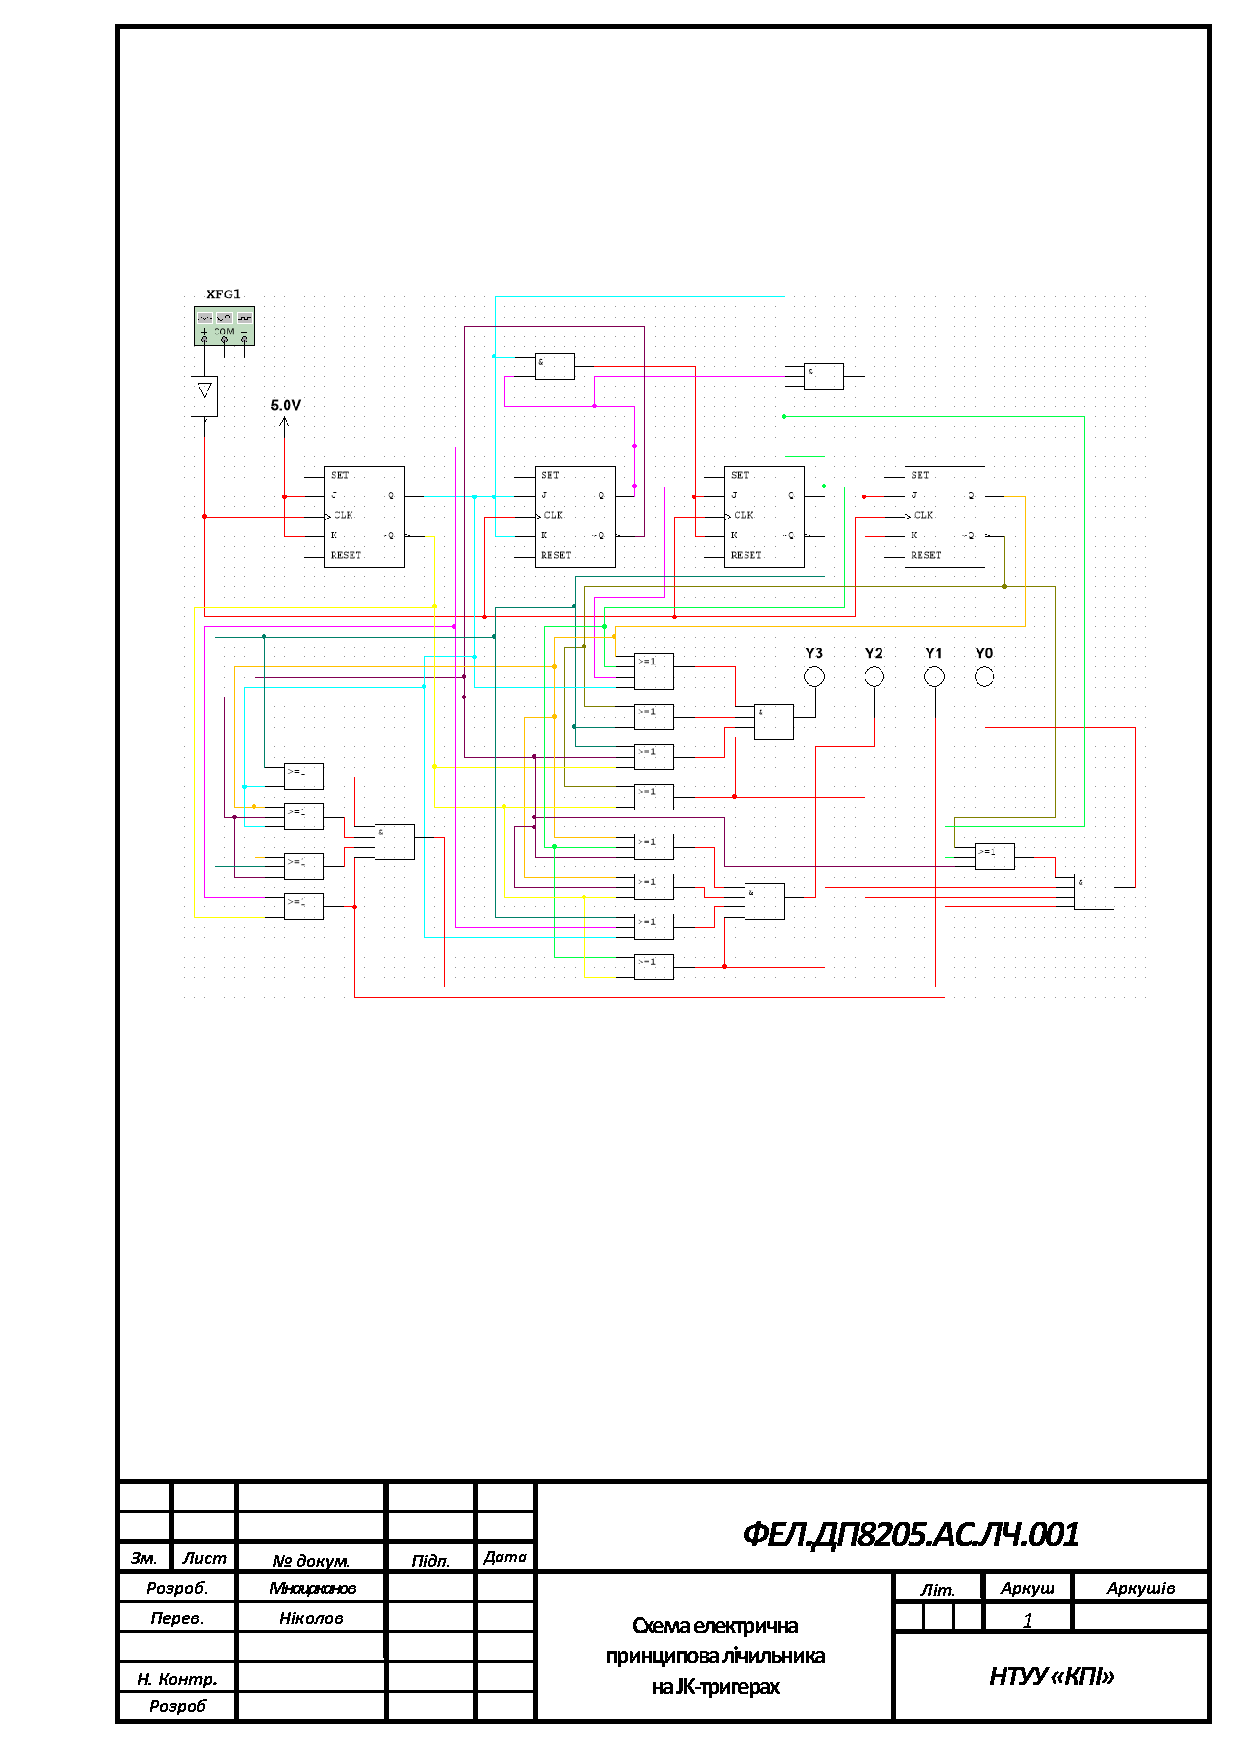
\includegraphics[width=1.0\linewidth]{sx.pdf}
\end{figure}



\end{document}
